\chapter{Quelltextausz�ge}
\index{a2ps}\index{Pretty Printer}\index{Quelltexte}

\textcolor{darkred}{Anmerkungen: Quelltextausz�ge zu einer Implementierung sind im Anhang dann sinnvoll, wenn einige, spezielle Implementierungstechniken aufgezeigt werden sollen, die in der Darstellung als Algorithmus oder Pseudocode nicht deutlich werden. Keinesfalls soll der gesamte Quelltext angeh�ngt werden und weiterhin soll auch in einer Vorbemerkung die Auswahl der Quelltextausz�ge genau erkl�rt werden.}

\textcolor{darkred}{Verwendet wird das freie Quelltext-Pretty-Printing-Tool a2ps.exe mit folgender Aufrufkonvention (vgl. \mbox{[a2ps 07, grep 07]):}}


\verb$     a2ps.exe --pretty-print=cxx -i test.cpp -o test.ps -T3$

\medskip
\medskip

\textcolor{darkred}{Die Quelltextdateien d�rfen hierf�r eine Zeilenl�nge von 80 nicht �berschreiten. Die st�renden Kommentare im Header und Footer des entstandenen .ps-Files k�nnen mithilfe des freien Tools grep.exe automatisiert entfernt werden. Eine Batch-Datei f�r den gesamten Konvertierungsprozess inklusive Konvertierung in das pdf-Format hat beispielsweise folgenden Inhalt:}


\verb$     a2ps --pretty-print=cxx -i %1 -o tmp -T3$\\
\verb$     grep -v "Gedruckt von" tmp | grep -v ") footer" > %1.ps$\\
\verb$     del tmp$\\
\verb$     "c:\programme\adobe\acrobat 7.0\Acrobat\acrobat.exe" %1.ps$\\

\textcolor{darkred}{Bei Adobe Acrobat Prof. 6.0 muss u.U. das Seitenformat korrigiert werden auf DIN-A4 = 210 mm$\times$ 297 mm, die Voreinstellung ist falsch (zu klein, ein Bug), zu korrigieren in: Bearbeiten / Grundeinstellungen / in pdf konvertieren / Postscript/EPS / Einstellungen bearbeiten / bearbeiten / Standardpapierformat. Weiterhin muss an der gleichen Stelle das korrekte und vollst�ndige Einbetten der Schriften eingestellt und sp�ter auch kontrolliert werden (vgl. Kapitel 1).}

Die nachfolgenden Quelltextausschnitte entstammen dem Programmmodul zum Lageausgleich. Der Quelltext ist hier im Anhang exemplarisch aufgenommen, da die Implementierung des Lageausgleiches auf Basis zentraler Momente f�r einige Leser von besonderem Interesse sein k�nnte.

Der Ausschnitt umfasst ca. 300 Programmzeilen, die gesamte im Rahmen der vorliegenden Arbeit entstandene Implementierung umfasst ca. 8.000 Programmzeilen.






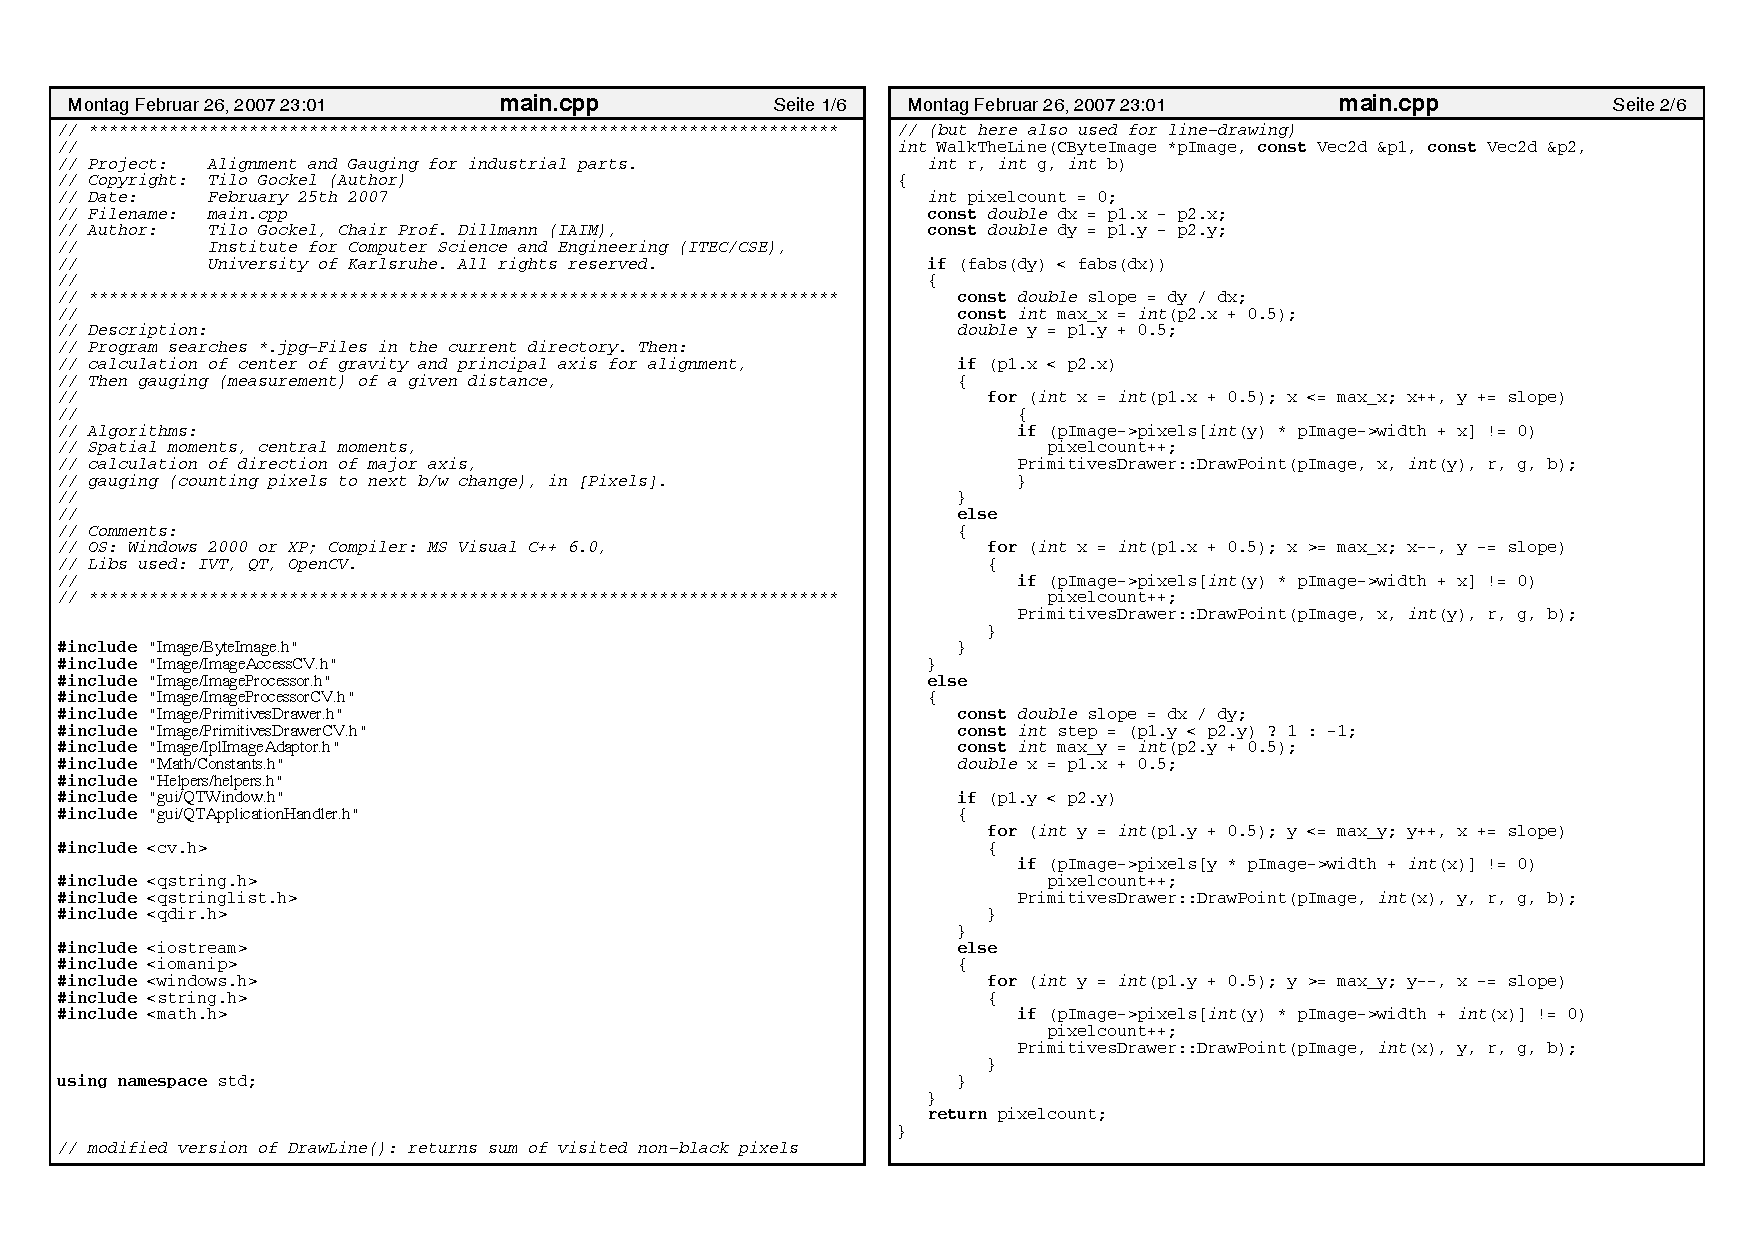
\includepdf[
 pages={-},
 nup=1x1,
 landscape=true,
 noautoscale=false,
 turn=false,
 scale=0.80,
 trim= 0mm 0mm 0mm 0mm,
 clip=true,
 pagecommand={},
 delta=0mm 0mm
]{BilderAnhangC/main_cpp.pdf}












